\documentclass[a4paper]{article}
\usepackage[spanish]{babel}
\usepackage[pdftex,usenames,dvipsnames]{color}
\usepackage{multicol}
\usepackage{graphicx}
\usepackage{listings}
\usepackage{color}

\definecolor{dkgreen}{rgb}{0,0.6,0}
\definecolor{gray}{rgb}{0.5,0.5,0.5}
\definecolor{mauve}{rgb}{0.58,0,0.82}

\lstset{
    language=bash, 
    basicstyle=\footnotesize\color{black},
    backgroundcolor=\color{white},
    morekeywords={durar}, keywordstyle=\color{green},
    classoffset=1,
    showspaces=false,
    showstringspaces=false,
    showtabs=false,
    frame=single, 
    tabsize=2,
    captionpos=b,
    breaklines=true,
}

\begin{document}
\pagestyle{plain}
\title{Práctica 3: Monitorización y "Profiling" \\ 
Ingeniería de Servidores}
\author{Raúl Durán Racero}
\begin{figure}
    \centering
    \includegraphics[width=1.25\textwidth]{servers.pdf}
\end{figure}
\maketitle
\begin{figure}
    \centering
    \includegraphics[width=0.25\textwidth]{logoEtsiit.pdf}
\end{figure}

\newpage
\tableofcontents
\newpage
\section{Ejercicio 1}
Realice una instalación de Zabbix 5.0 en su servidor con \textbf{Ubuntu Server20.04} y configure
para que se monitorice a él mismo y para que monitorice a la máquina con \textbf{CentOS}.
Puede configurar varios parámetros para monitorizar, uso de CPU, memoria, etc. pero
debe configurar de manera obligatoria la monitorización de los servicios \textbf{SSH} y \textbf{HTTP}.
\subsection{Instalación de Zabbix}
Por comodidad a la hora de instalar, me conectaré a la máquina virtual de UbuntuServer
a través de SSH, para poder copiar algunos comandos que son muy largos.\newline
Lo primero que tenemos que hacer es instalar Zabbix en Ubuntu. Para ello, 
descargamos su paquete:

\begin{lstlisting}
    durar@durar:~$ wget https://repo.zabbix.com/zabbix/5.0/ubuntu/pool/main/z/zabbix-release/zabbix-release_5.0-1+focal_all.deb
\end{lstlisting}
Una vez descargado, lo instalamos con \textsl{dpkg -i} y obtenemos las actualizaciones
con \textsl{apt update} (es necesario tener permisos de superusuario):
\begin{lstlisting}
    durar@durar:~$ sudo dpkg -i zabbix-release_5.0-1+focal_all.deb
    durar@durar:~$ sudo apt update
\end{lstlisting}
Nos falta instalar el servidor, la interfaz y el agente de Zabbix:
\begin{lstlisting}
    durar@durar:~$ sudo apt install zabbix-server-mysql zabbix-frontend-php zabbix-apache-conf zabbix-agent
\end{lstlisting}
Ya tenemos todo debidamente instalado, por lo que pasaremos a crear una base de 
datos inicial y un usuario, dándole todos los permisos (entraré en mysql como superusuario ya que no 
me permite entrar con \textsl{mysql -u root -p}).
\begin{lstlisting}
    durar@durar:~$ sudo mysql 
    mysql> create database zabbix character set utf8 collate utf8_bin;
    mysql> create user zabbix@localhost identified by 'password';
    mysql> grant all privileges on zabbix.* to zabbix@localhost;
    mysql> quit;
\end{lstlisting}
A continuación tenemos que ejectuar el script que establece el esquema por defecto de 
la base de datos.
\begin{lstlisting}
    durar@durar:~$ zcat /usr/share/doc/zabbix-server-mysql*/create.sql.gz | mysql -uzabbix -p zabbix
\end{lstlisting}
Esto puede tardar un tiempo. Podemos comprobar que se está ejecutando con \textsl{htop}
desde la máquina de UbuntuServer:
\begin{figure}
    \centering
    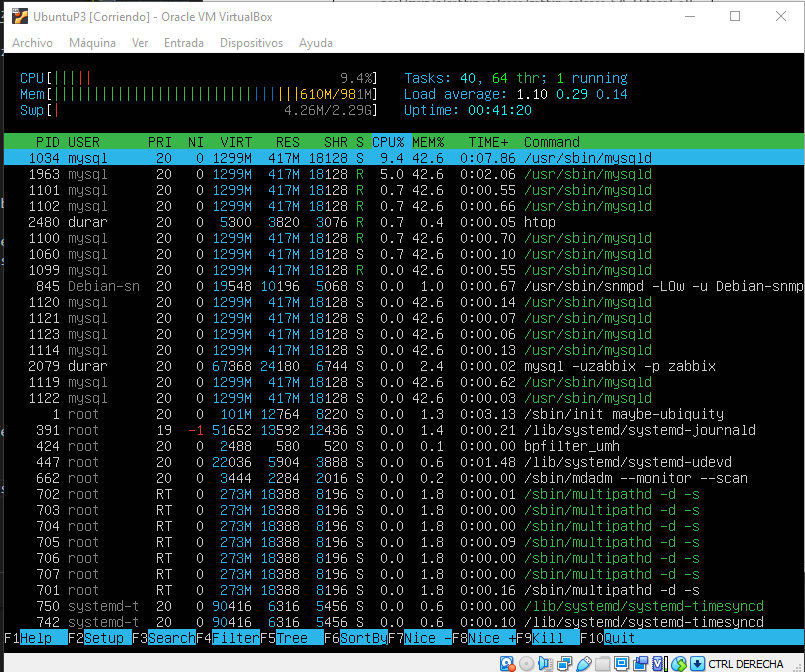
\includegraphics[width=1.0\textwidth]{htop de mysql.png}
\end{figure}
\newpage
Puede verse que efectivamente mysql está en ejecución.\newline
Ya tenemos la base de datos creada, así que ahora toca configurarla.
Primero, editamos el archivo /etc/zabbix/zabbix\_server.conf:
\begin{lstlisting}
    durar@durar:~$ sudo vi /etc/zabbix/zabbix_server.conf
\end{lstlisting}
Y ponemos nuestra contraseña en la línea donde está \textbf{DBPassword}: 
\begin{lstlisting}
    DBPassword=ISE
\end{lstlisting}
Para buscar la línea, se puede usar \textbf{Shift+7} en vi para buscar DBPassword más 
facilmente.
\end{document}